\documentclass[10pt]{article}
\usepackage[utf8]{inputenc}
\usepackage{mathtools}
\usepackage{graphicx}
\usepackage{array}
\usepackage[margin=0.5in]{geometry}
\usepackage{listings}
\usepackage{color}

\definecolor{mygreen}{rgb}{0,0.6,0}
\definecolor{mygray}{rgb}{0.5,0.5,0.5}
\definecolor{mymauve}{rgb}{0.58,0,0.82}

\lstset{ %
  backgroundcolor=\color{white},   % choose the background color; you must add \usepackage{color} or \usepackage{xcolor}; should come as last argument
  basicstyle=\footnotesize,        % the size of the fonts that are used for the code
  breakatwhitespace=false,         % sets if automatic breaks should only happen at whitespace
  breaklines=true,                 % sets automatic line breaking
  captionpos=b,                    % sets the caption-position to bottom
  commentstyle=\color{mygreen},    % comment style
  deletekeywords={...},            % if you want to delete keywords from the given language
  escapeinside={\%*}{*)},          % if you want to add LaTeX within your code
  extendedchars=true,              % lets you use non-ASCII characters; for 8-bits encodings only, does not work with UTF-8
  frame=single,	                   % adds a frame around the code
  keepspaces=true,                 % keeps spaces in text, useful for keeping indentation of code (possibly needs columns=flexible)
  keywordstyle=\color{blue},       % keyword style
  language=Octave,                 % the language of the code
  morekeywords={*,...},            % if you want to add more keywords to the set
  numbers=left,                    % where to put the line-numbers; possible values are (none, left, right)
  numbersep=5pt,                   % how far the line-numbers are from the code
  numberstyle=\tiny\color{mygray}, % the style that is used for the line-numbers
  rulecolor=\color{black},         % if not set, the frame-color may be changed on line-breaks within not-black text (e.g. comments (green here))
  showspaces=false,                % show spaces everywhere adding particular underscores; it overrides 'showstringspaces'
  showstringspaces=false,          % underline spaces within strings only
  showtabs=false,                  % show tabs within strings adding particular underscores
  stepnumber=2,                    % the step between two line-numbers. If it's 1, each line will be numbered
  stringstyle=\color{mymauve},     % string literal style
  tabsize=2,	                   % sets default tabsize to 2 spaces
  title=\lstname                   % show the filename of files included with \lstinputlisting; also try caption instead of title
}
\renewcommand{\arraystretch}{1.5}
\setcounter{secnumdepth}{0}
\author{Kevin Mambu}
\date{\today}

\title{M1 SESI 2017-2018\\Architecture Multi-Processeurs\\TP2 : Architecture
Interne du Contrôleur de Cache}

\begin{document}
\maketitle

\section{Spécifications}

\section{Question C1}
L'adresse de la première instruction du main est 0x00400000. La quatrième
instruction du main est l'instruction du loop, à 0x0040000c.

\section{Question C2}
\begin{itemize}
  \item A est la première structure en mèmoire du segment data, donc\\
  @A : 0x01000000
  \item @B : $@A+20\times4+48$ = 0x01000080
  \item @C : $@B+20\times4+48$ = 0x01000100
\end{itemize}

\section{Question C3}
Parce que le MIPS32 est un processeur pipeline 5 étages et qu'à cause du plan
pipeline de ce processeur, lors d'un branchement, l'instruction suivante est
systématiquement exécutée, sinon on ne peut pas calculer l'adresse après le
branchement. On met en temps normal un delayed slot (nop) pour faire face à
cette contrainte mais mettre le sw à cette endroit est une optimisation.

\section{Question C4}
Considérons que la boucle d'itération soit suffisament longue en nombre
d'instructions pour que le TEP ne congéstionne pas au {\it sw} de chaque
itération, chaque instruction serait exécutée son cycle, car aucun MISS ne
serait présent. Donc 7 instructions par itération de boucle.

\section{Question D1}
\begin{itemize}
  \item 1 ligne de cache est composée de 16 octets. ${BYTE}=log_2(16)=4$ bits
  \item Le cache est à correspondance directe $\rightarrow$ 1 case accessible
  par ligne.\\
  ${SET}=log_2(\frac{128}{16})=3$ bits.
  \item ${TAG}=32-(3+4)=25$ bits.
\end{itemize}

\section{Question D2}
Le premier MISS d'instruction est le MISS mandataire pour le chargement du code
du {\it main} :
\lstinputlisting[firstline=8,lastline=8]{app.bin.txt}
\begin{tabular}{|c|c|c|c|c|c|c|}
  \hline
  \#ligne & valide? & tag & mot3 & mot2 & mot1 & mot0 \\ \hline
  7 & 0 & & & & & \\ \hline
  6 & 0 & & & & & \\ \hline
  5 & 0 & & & & & \\ \hline
  4 & 0 & & & & & \\ \hline
  3 & 0 & & & & & \\ \hline
  2 & 1 & 0x$004000_{0}$ & 0x3c040040 & 0xad0c00fc & 0x14c7fffa & 0x014b6020 \\ \hline
  1 & 1 & 0x$004000_{0}$ & 0x21080004 & 0x20c60001 & 0x8d0b0080 & 0x8d0a0000 \\ \hline
  0 & 1 & 0x$004000_{0}$ & 0x24060000 & 0x24070014 & 0x25080080 & 0x3c080100 \\ \hline
\end{tabular}\\
Soit 3 MISS d'instructions.

\section{Question D3}
Avant la première instruction de la boucle, on peut comptabiliser deux MISS.\\
Parce que toutes les instructions de la boucles sont en mémoire cache après la
première itération, à terme de la 20e itération, le contenu du cache
d'instruction est inchangé depuis la fin de la première itération.\\
Au total, on comptabilise 5 MISSes pour ${10}+{20}\times{7}={150}$
instructions.\\
$\tau_{MISS}=\frac{5}{150}\approx0.033\%$

\section{Question D4}
L'état MISS\_SELECT est indispensable pour un cache associatif, parce qu'en
dehors du cas d'un cache à correspondance directe, il est possible pour une
ligne de cache d'être rangée dans une case du cache parmi plusieurs emplacements
possibles.

\section{Question D5}
\begin{center}
  \begin{tabular}{|c|c|}
    \hline
    {\bf Transition} & {\bf Expression} \\ \hline
    {\bf A} & ${IMISS}\bullet{IUNC}$ \\ \hline
    {\bf B} & ${IMISS}\bullet\overline{IUNC}$ \\ \hline
    {\bf C} & $\overline{IMISS}$ \\ \hline
    {\bf I} & $1$ \\ \hline
    {\bf F} & ${IREQ}\bullet{VALID}\bullet\overline{ERROR}$ \\ \hline
    {\bf G} & ${IREQ}\bullet{VALID}\bullet{ERROR}$ \\ \hline
    {\bf H} & $\overline{IREQ}+\overline{VALID}$ \\ \hline
    {\bf N} & $1$ \\ \hline
    {\bf L} & ${IREQ}\bullet{VALID}\bullet\overline{ERROR}$ \\ \hline
    {\bf K} & ${IREQ}\bullet{VALID}\bullet{ERROR}$ \\ \hline
    {\bf J} & $\overline{IREQ}+\overline{VALID}$ \\ \hline
    {\bf M} & $1$ \\ \hline
    {\bf O} & $1$ \\ \hline
  \end{tabular}
\end{center}

\section{Question D6}
Le signal RESETN doit forcer l'automate du cache d'instruction à l'état IDLE
pour qu'il soit prêt à recevoir la première requête du processeur: charger le
code du bootloader depuis la ROM. L'autre effet qui se coule est que le cache
doit être prêt à recevoir de l'information sur l'intégralité de sa mémoire, donc
l'intégralité du cache doit être invalidé.

\section{Question E1}
Voici les champs des adresses de A[0] et B[0] :
\begin{tabular}{|c|c|c|c|c|}
  \hline
 & Adresse & TAG & SET & BYTE \\ \hline
 A & 0x01000000 & 0x$010000_0$ & 0 & 0 \\ \hline
 B & 0x01000080 & 0x$010000_1$ & 0 & 0 \\ \hline
\end{tabular}
Les deux instructions générant des MISSes sont les suivantes :
\lstinputlisting[firstline=14,lastline=15]{app.bin.txt}
La première génere un MISS compulsif car la donnée n'est pas présente en
mémoire, tous les MISSes suivants génèrent des MISSes de conflits, alors que
les valeurs de A vont écraser les valeurs de B.\\
\begin{tabular}{|c|c|c|c|c|c|c|}
  \hline
  \#ligne & valide? & tag & mot3 & mot2 & mot1 & mot0 \\ \hline
  7 & 0 & & & & & \\ \hline
  6 & 0 & & & & & \\ \hline
  5 & 0 & & & & & \\ \hline
  4 & 0 & & & & & \\ \hline
  3 & 0 & & & & & \\ \hline
  2 & 0 & & & & & \\ \hline
  1 & 0 & & & & & \\ \hline
  0 & 1 & 0x$0100000_1$ & 104 & 103 & 102 & 101 \\ \hline
\end{tabular}\\
Soit deux MISSes par itération de boucle.

\section{Question E2}
On comptabilise à terme ${2}\times{20}={40}$ MISSes de données.\\Voici l'état du
cache à la 20e itération:\\
\begin{tabular}{|c|c|c|c|c|c|c|}
  \hline
  \#ligne & valide? & tag & mot3 & mot2 & mot1 & mot0 \\ \hline
  7 & 0 & & & & & \\ \hline
  6 & 0 & & & & & \\ \hline
  5 & 0 & & & & & \\ \hline
  4 & 1 & 0x$0100000_1$ & 120 & 119 & 118 & 117 \\ \hline
  3 & 1 & 0x$0100000_1$ & 116 & 115 & 114 & 113 \\ \hline
  2 & 1 & 0x$0100000_1$ & 112 & 111 & 110 & 109 \\ \hline
  1 & 1 & 0x$0100000_1$ & 108 & 107 & 106 & 105 \\ \hline
  0 & 1 & 0x$0100000_1$ & 104 & 103 & 102 & 101 \\ \hline
\end{tabular}

\section{Question E3}
\begin{center}
  \begin{tabular}{|c|c|}
    \hline
    {\bf Transition} & {\bf Expression} \\ \hline
    {\bf A} & ${DMISS}\bullet{DUNC}\bullet\overline{WRITE}$ \\ \hline
    {\bf B} & ${DMISS}\bullet\overline{DUNC}\bullet\overline{WRITE}$ \\ \hline
    {\bf C} & $\overline{DMISS}+\overline{WRITE}$ \\ \hline
    {\bf I} & $1$ \\ \hline
    {\bf F} & ${IREQ}\bullet{VALID}\bullet\overline{ERROR}$ \\ \hline
    {\bf G} & ${IREQ}\bullet{VALID}\bullet{ERROR}$ \\ \hline
    {\bf H} & $\overline{IREQ}+\overline{VALID}$ \\ \hline
    {\bf N} & $1$ \\ \hline
    {\bf L} & ${IREQ}\bullet{VALID}\bullet\overline{ERROR}$ \\ \hline
    {\bf K} & ${IREQ}\bullet{VALID}\bullet{ERROR}$ \\ \hline
    {\bf J} & $\overline{IREQ}+\overline{VALID}$ \\ \hline
    {\bf M} & $1$ \\ \hline
    {\bf O} & $1$ \\ \hline
    {\bf D} & ${WRITE}\bullet\overline{WOK}$ \\ \hline
    {\bf P} & $1$ \\ \hline
    {\bf E} & ${WRITE}\bullet{WOK}$ \\ \hline
  \end{tabular}
\end{center}

\section{Question E4}
[TODO]

\section{Question F1}
Les écritures ont une priorité plus élevée pour assurer le vidage du TEP.

\section{Question F2}
Afin d'assurer la communication client/serveur, un système de deux bascules RS
est employé. Le client, après préparation de sa requête met à SET la bascule
REQ, qui sera remis à RESET par le serveur pour prévenir le client de
l'aquittement de la requête.\\
Le serveur, après le transfert, met la bascule RSP à SET pour prévenir le client
de la fin de la transaction. Le client lui, la met à RESET pour prévenir le
serveur de l'aquittement de la réponse.

\section{Question F3}
[TODO]

\section{Question F4}
\begin{tabular}{|c|c|}
  \hline
  {\bf Transition} & {\bf Expression} \\ \hline
  Y & $({IUNC}+{IMISS})\bullet\overline{ROK}\bullet\overline{SC}$ \\ \hline
  Y & $({DUNC}+{DMISS})\bullet\overline{ROK}\bullet\overline{SC}$ \\ \hline
  Z & $\overline{{IUNC}+{IMISS}+{DUNC}+{DMISS}+{ROK}+{SC}}$ \\ \hline
  B' & $\overline{GNT}$ \\ \hline
  B & ${GNT}$ \\ \hline
  E' & $\overline{GNT}$ \\ \hline
  E & ${GNT}$ \\ \hline
  C & $1$ \\ \hline
  D' & ${{ACK}\oplus{WAIT}}$ \\ \hline
  D & $\overline{{ACK}\oplus{WAIT}}$ \\ \hline
  H' & ${{ACK}\oplus{WAIT}}$ \\ \hline
  H & $\overline{{ACK}\oplus{WAIT}}$ \\ \hline
  F' & $\overline{LAST}$ \\ \hline
  F & ${LAST}$ \\ \hline
  G' & $\overline{LAST}$ \\ \hline
  G & ${LAST}$ \\ \hline
\end{tabular}

\section{Question F5}
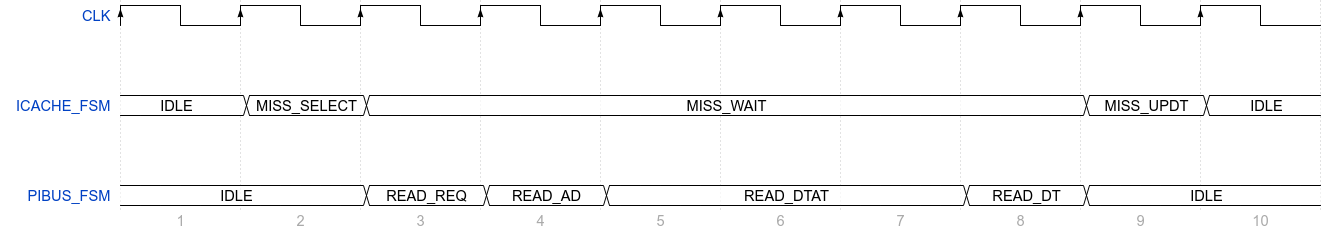
\includegraphics[width=18cm]{icache_wave.png}\\
L'évolution des états internes du DCACHE\_FSM est identique à celle représentée
ci-dessus pour une lecture. 9 cycles de gel en cas de MISS dans les deux cas.

\section{Question F6}
À la première itération on comptabilise deux MISS d'instruction compulsifs.\\
À toutes les itérations on comptabilise deux MISS de données dûs aux conflits.\\
Sachant que le poids du MISS est de 9 cycles de gel :
\begin{itemize}
  \item $\#cycle=(\underbrace{2\times{10}}_{imiss}+
    \underbrace{2\times{10}}_{dmiss}+5)+
    {19}\times\underbrace{2\times{10}}_{dmiss}+5=525$ cy
  \item ${CPI}=\frac{525}{140}=3.75$!
\end{itemize}

\section{Question G1}
La première instruction s'exécute au cycle 10 :
\lstinputlisting[firstline=280,lastline=301]{trace.txt}
Cela correspond à la première instruction du segment {\it seg\_reset}. Pendant
les dix premiers cycles (du cycle 0 au cycle 9), le processeur est gelé. On
retrouve bien la valeur théorique du nombre de cycles de gel pour un MISS
d'instruction.

\section{Question G2}
Le branchement vers la première instruction du {\bf main} est :
\lstinputlisting[firstline=17,lastline=17]{sys.bin.txt}
La commande eret passe du code système au code utilisateur via un branchement
à l'adresse stockée dans le registre EPC (au démarrage de la machine, la valeur
de EPC est à 0x00400000). Le branchement se fait au cycle 46 :
\lstinputlisting[firstline=1072,lastline=1093]{trace.txt}

\section{Question G3}
On remarque en observant la trace qu'une lecture de donnée non en cache au
cycle 71 prend jusqu'au cycle 81 pour être menée, soit 10 cycles. En enlevant
la requête, le coût du MISS est de 9 cycles.
La première itération commence au cycle 71 et se termine au cycle 107, soit
36 cycles :
\newpage
\lstinputlisting[firstline=1622,lastline=1643]{trace.txt}
\lstinputlisting[firstline=2414,lastline=2435]{trace.txt}
\newpage

\section{Question G4}
La seconde et troisième itération prennent chaqu'une 30 cycles. Le coût des
MISSes de données sont plus importants parce qu'il faut maintenant invalider la
ligne de cache dans la case où on veut charger la nouvelle ligne depuis la
mémoire.

\end{document}
